\documentclass[hyperref=colorlinks]{beamer}
\mode<presentation>
\usetheme{iclpt}
\setbeamertemplate{navigation symbols}{}
\setbeamertemplate{headline}{
\begin{beamercolorbox}[leftskip=.2cm,rightskip=.2cm,topskip=.2cm,ht=1.1cm,dp=0.1cm,wd=\textwidth]{institute in head/foot}
  
\includegraphics[height=1cm]{icl.pdf}
  \hfill
  
\includegraphics[height=1cm]{../Pics/CMS-Color.pdf}
\end{beamercolorbox}
}
\setbeamertemplate{footline}{
\begin{beamercolorbox}[ht=.55cm,dp=0.4cm,wd=\textwidth,leftskip=.3cm]{author in head/foot}%
  \begin{minipage}[c]{5cm}%
    \usebeamerfont{author in head/foot}
    \insertshortauthor 
    \insertshorttitle
    \end{minipage}\hfill%
  \insertframenumber{} / \pageref{lastframe}
  \hfill
  \begin{minipage}{6cm}
    \hfill
  \end{minipage}
\end{beamercolorbox}%
}

\usepackage{color}
\usepackage{tabularx,colortbl}
\usepackage{graphicx}
\usepackage{pdfpages}
\usepackage{feynmp}
\usepackage{tikz}
\usetikzlibrary{calc, shapes, backgrounds,arrows,positioning}
\DeclareGraphicsRule{*}{mps}{*}{}

\title{\vspace{-0.2cm} Imperial College - Dimuon bump cross check}
\subtitle{\vspace{-0.7cm}}
\author[]{}%\underline{P. Dunne}} % A.M. Magnan and A. Nikitenko Joao Pela with \\ R. Aggleton, J. Brooke: Bristol \\ C.Asawangtrakuldee, Q.Li: Peking \\ P. Srimanobhas: Chulalongkorn \\ S. Kumar, K. Mazumdar: Mumbai}
\titlegraphic{
  \vspace{-0.7cm}
  %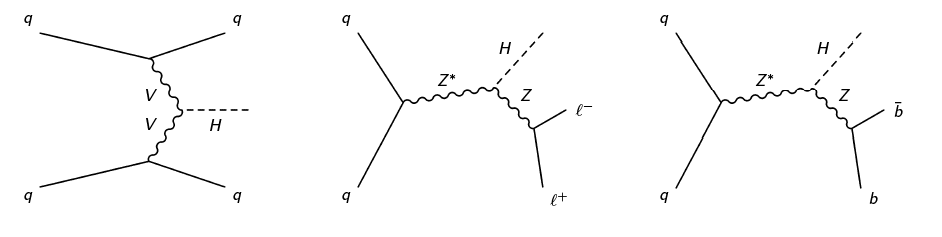
\includegraphics[width=\textwidth]{TalkPics/invcomb021213/feyndiags}
  %% \begin{fmfgraph*}(100,70)
  %%         \fmfleft{i1,i2}
  %%         \fmfright{o1,o2,o3}
  %%         \fmf{fermion}{i1,v1,o1}
  %%         \fmf{fermion}{i2,v2,o3}
  %%         \fmf{phantom,tension=4/5}{v1,v2}
  %%         \fmffreeze
  %%         \fmf{photon,label=$W,,Z$}{v1,v3}
  %%         \fmf{photon,label=$W,,Z$}{v2,v3}
  %%         \fmf{dashes}{v3,o2}
  %%         \fmflabel{$q$}{i1}
  %%         \fmflabel{$q$}{i2}
  %%         \fmflabel{$q$}{o1}
  %%         \fmflabel{$q$}{o3}
  %%         \fmflabel{$H$}{o2}
  %%       \end{fmfgraph*}
}
\date{}
\begin{document}
\begin{fmffile}{higgsexoupdatefeyndiags}
\tikzstyle{every picture}+=[remember picture]

%TITLE PAGE
\section{Title}
\begin{frame}
  \titlepage
  
\end{frame}

\begin{frame}
  \frametitle{Introduction}
  \begin{block}{}
    \begin{itemize}
    \item A bump in the dimuon mass spectrum was presented to this meeting several weeks ago
    \item The VBF H$\rightarrow$invisible group have the full single mu primary dataset processed for our trigger efficiency studies
    \item[-] Ntuples have no skimming so all events are present
    \item We have cross-checked the original analysis:
    \item[-] Common framework and ntuple format with Imperial H$\rightarrow\tau\tau$ has been used
    \end{itemize}
    \end{block}
\end{frame}

\begin{frame}
  \frametitle{Object ID}
  %!!MuScle, PF vs Trk Iso, PU ID, trigger
  \centering
  \begin{block}{}
    \begin{tabular}{|l|c|c|}
      \hline
      & Original analysis & IC crosscheck \\
      \hline
      \hline
      Data & \multicolumn{2}{|c|}{22Jan2013 ReReco} \\
      \hline
      Global Tag & \multicolumn{2}{|c|}{FT53\_V21A\_AN6} \\
      \hline
      Trigger & \multicolumn{2}{|c|}{HLT\_IsoMu24\_eta2p1 or HLT\_IsoMu24} \\
      \hline
      Muon isolation & Track iso$<0.1$ & PF iso$<0.2$ \\
      \hline
      MuScle Fit applied & Yes & No \\
      \hline
      Muon-jet overlap & 5 GeV & 10 GeV \\
      pt threshold & & \\
      \hline
      PU ID version & 52X & 53X \\
      \hline
      b-tagging & CSVMVA$>$0.783 & CSV$>$0.898 \\
      \hline
    \end{tabular}
  \end{block}

\end{frame}

\begin{frame}
  \frametitle{Selection}
  \begin{block}{}
    \begin{tabular}{lc}
      \hline
      Step name & Cuts \\
      \hline
      \hline
      Muon pair & Two OS muons,$\mu_{1}\, p_{T}>25$ GeV, \\
      & $\mu_{2}\, p_{T}>25$ GeV \\
      \hline
      Any central jet & At least one jet, $p_{T}>30$ GeV, \\
      & $|\eta|<2.4$ \\
      \hline
      Any central b jet & At least one jet, $p_{T}>30$ GeV, \\
      & $|\eta|<2.4$, CSV$>$0.898 \\
      \hline
      Other central jet veto (CJV) & Only one jet, $p_{T}>30$ GeV,\\
      & $|\eta|<2.4$ \\
      \hline
      Forward jet & At least one jet, $p_{T}>30$ GeV, \\
      & $|\eta|>2.4$ \\
      \hline
      Mass window & $26<M_{\mu\mu}>32$ GeV \\
      \hline
    \end{tabular}
  \end{block}
\end{frame}

\begin{frame}
  \frametitle{Cut flow}
  \centering
  \vspace{-.2cm}
  \begin{block}{}
    \begin{itemize}
    \item Yields compared at each cut step
    \item IC crosscheck yield close but consistently slightly lower
    \item At final step IC crosscheck has 23/28 events in common
    \item[-] 5 events present not in original analysis
    \item[-] 10 events in original analysis don't pass our selection
    \end{itemize}
    \centering
    \begin{tabular}{|l|c|c|}
      \hline
      Cut step & Original analysis & IC crosscheck \\
      \hline
      Muon pair & 162483 & 138364 \\
      Any central jet & 56788 & 41796 \\
      Any centrol b jet & 4286 & 4111 \\
      Other central jet veto & 1190 & 1055 \\
      Forward jet & 186 & 163 \\
      Mass window & 33 & 28 \\
      \hline
    \end{tabular}
  \end{block}
\end{frame}

\begin{frame}
  \frametitle{Dimoun mass distributions - Muon pair}
  \centering
  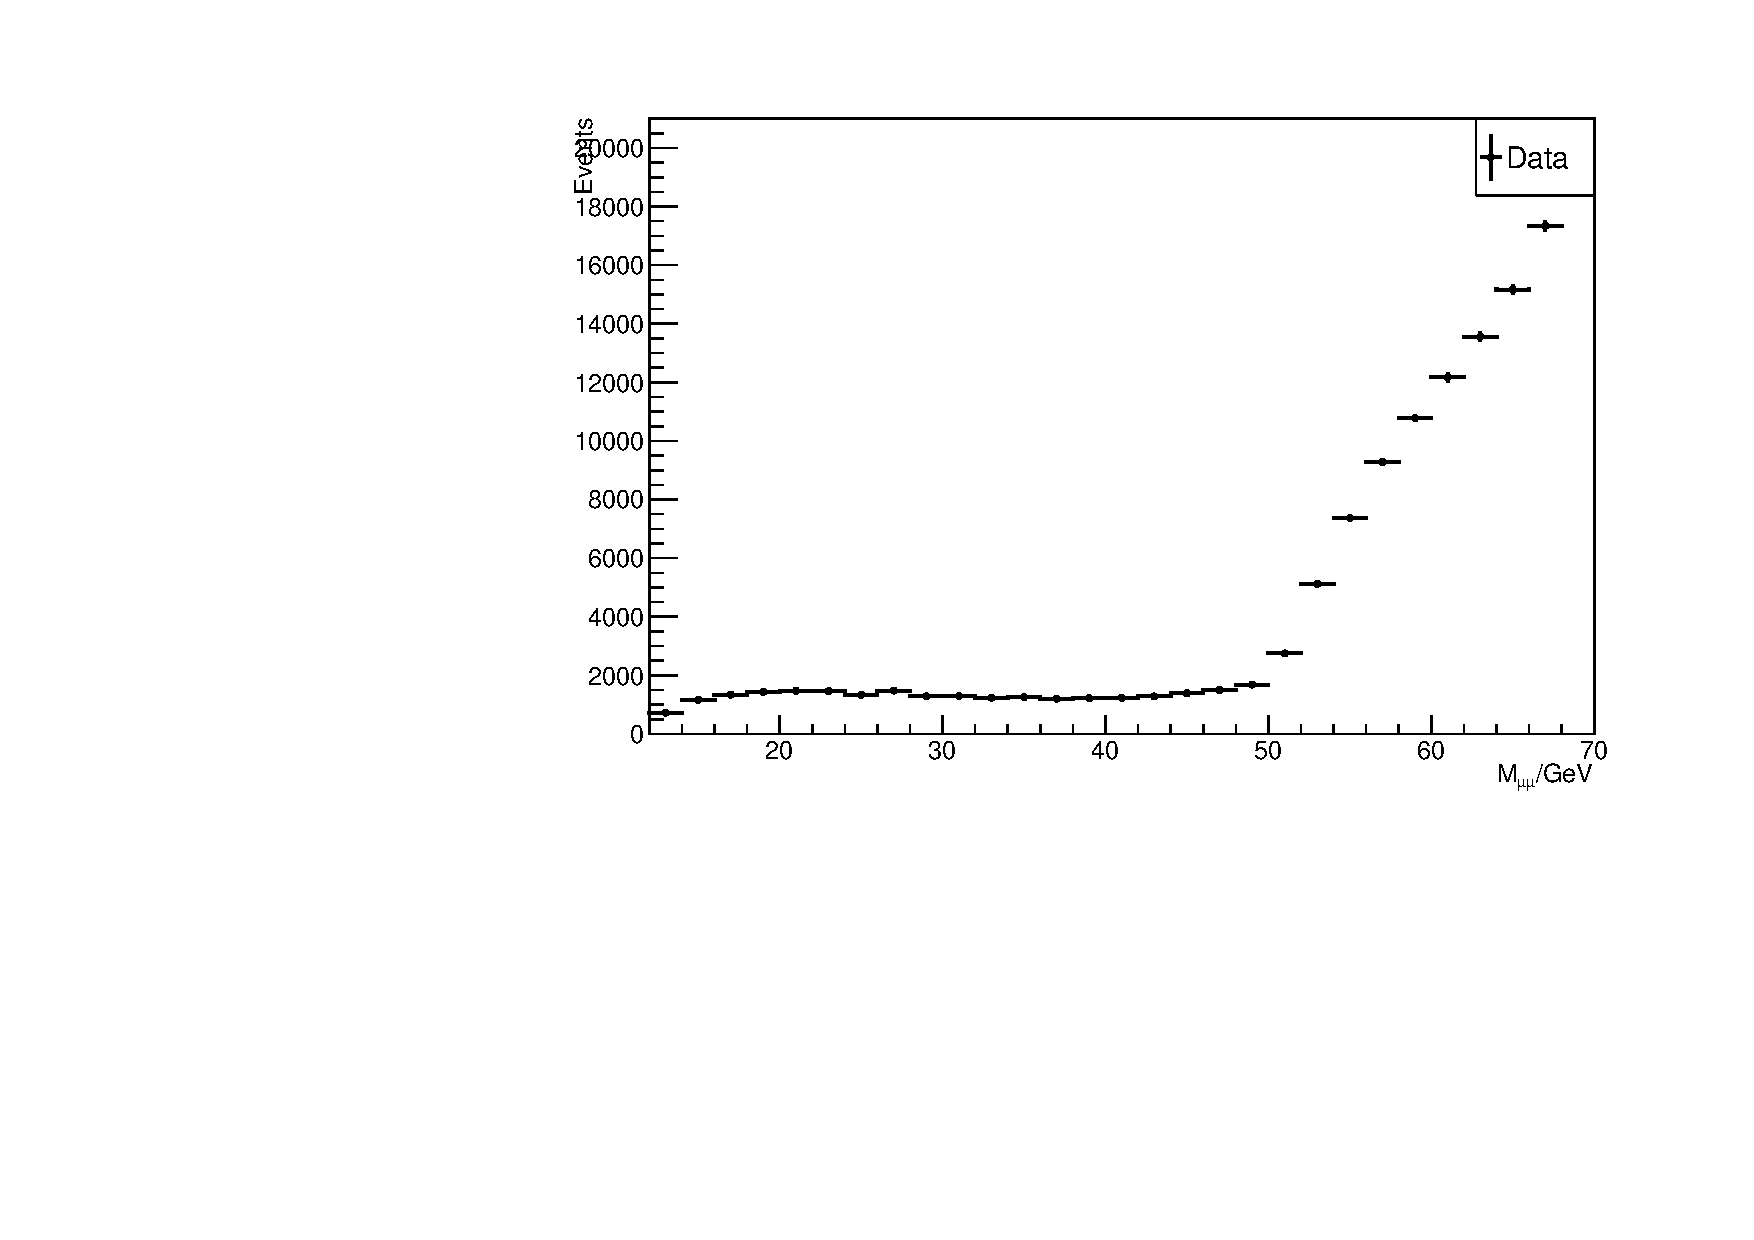
\includegraphics[width=.8\textwidth]{TalkPics/dimuoncheck100815/output_sashacheck_bugfixcsvtight/mmumu_mupair.pdf}
\end{frame}

\begin{frame}
  \frametitle{Dimoun mass distributions - Any central jet}
  \centering
  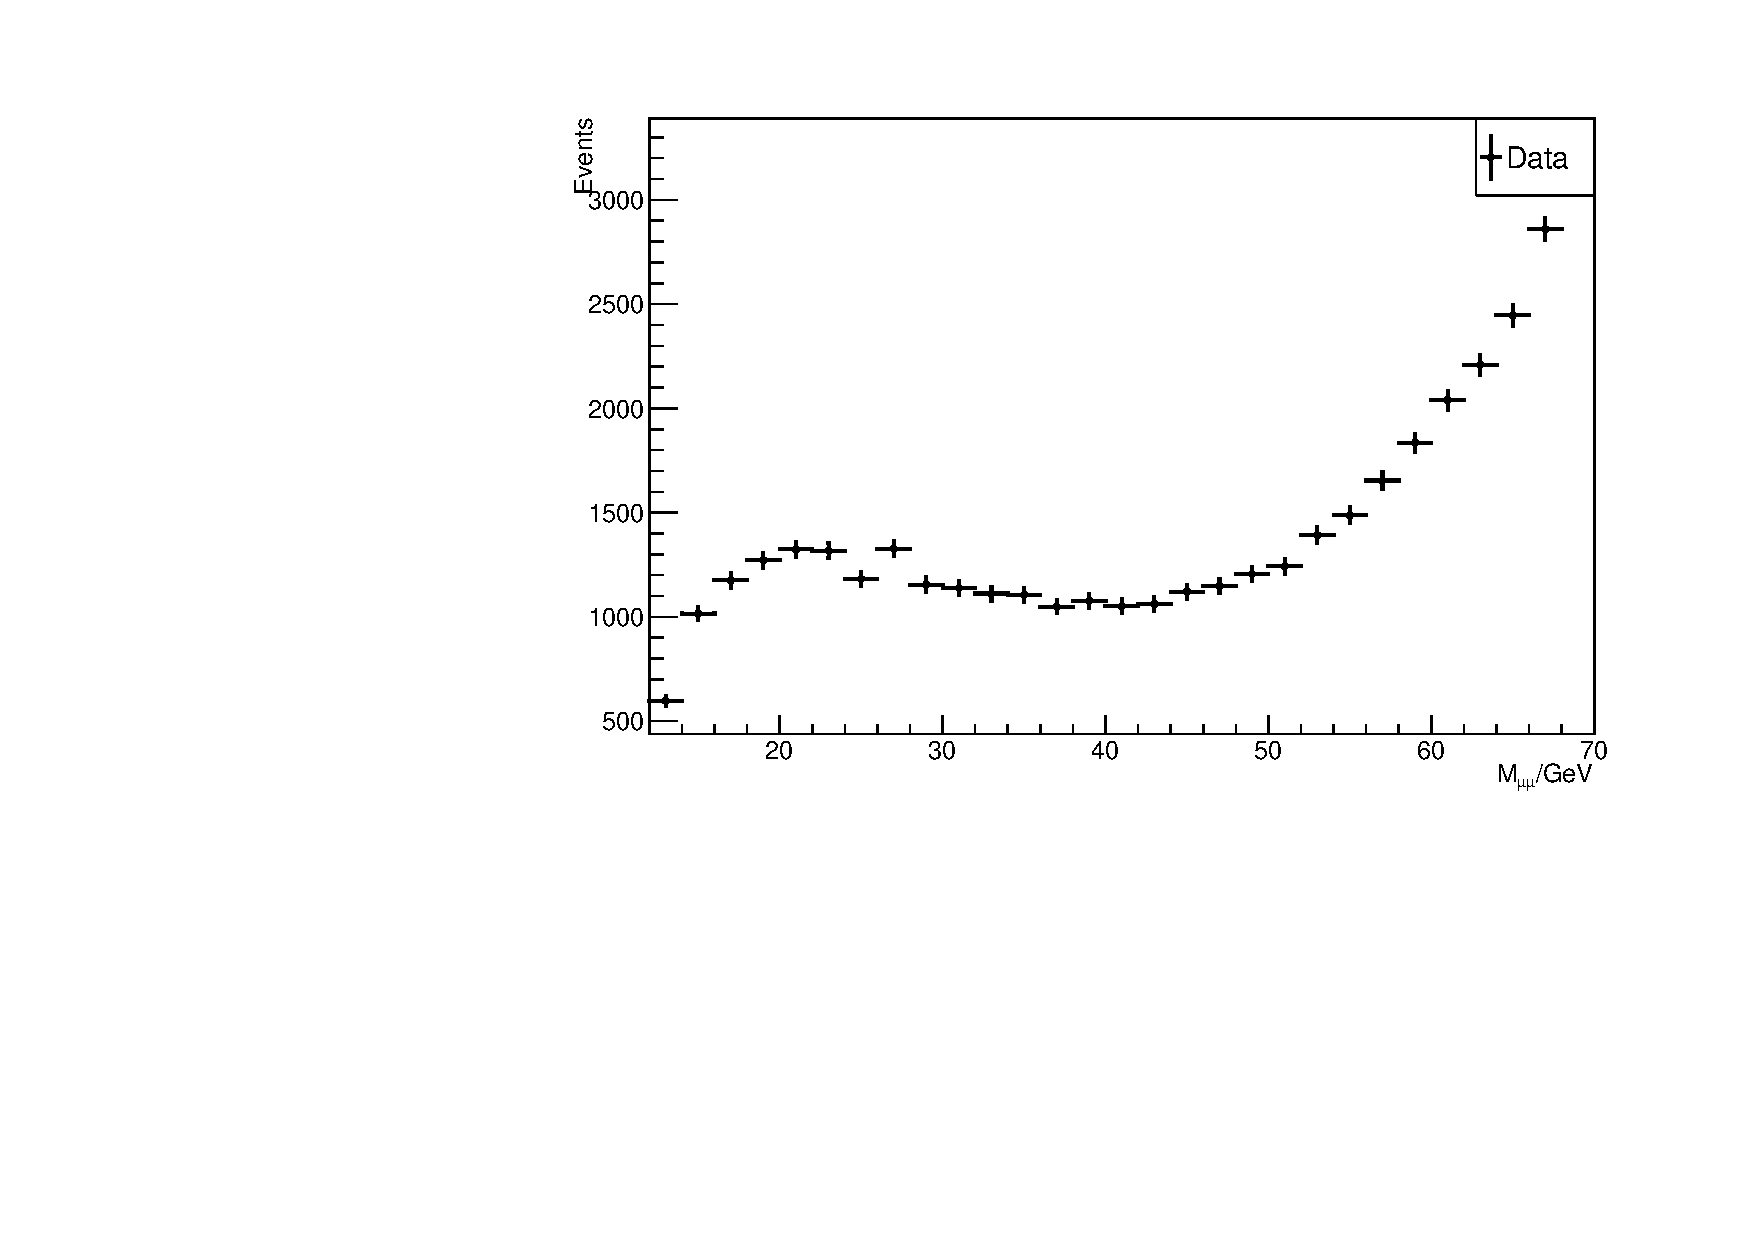
\includegraphics[width=.8\textwidth]{TalkPics/dimuoncheck100815/output_sashacheck_bugfixcsvtight/mmumu_centraljet.pdf}
\end{frame}

\begin{frame}
  \frametitle{Dimoun mass distributions - Any central b jet}
  \centering
  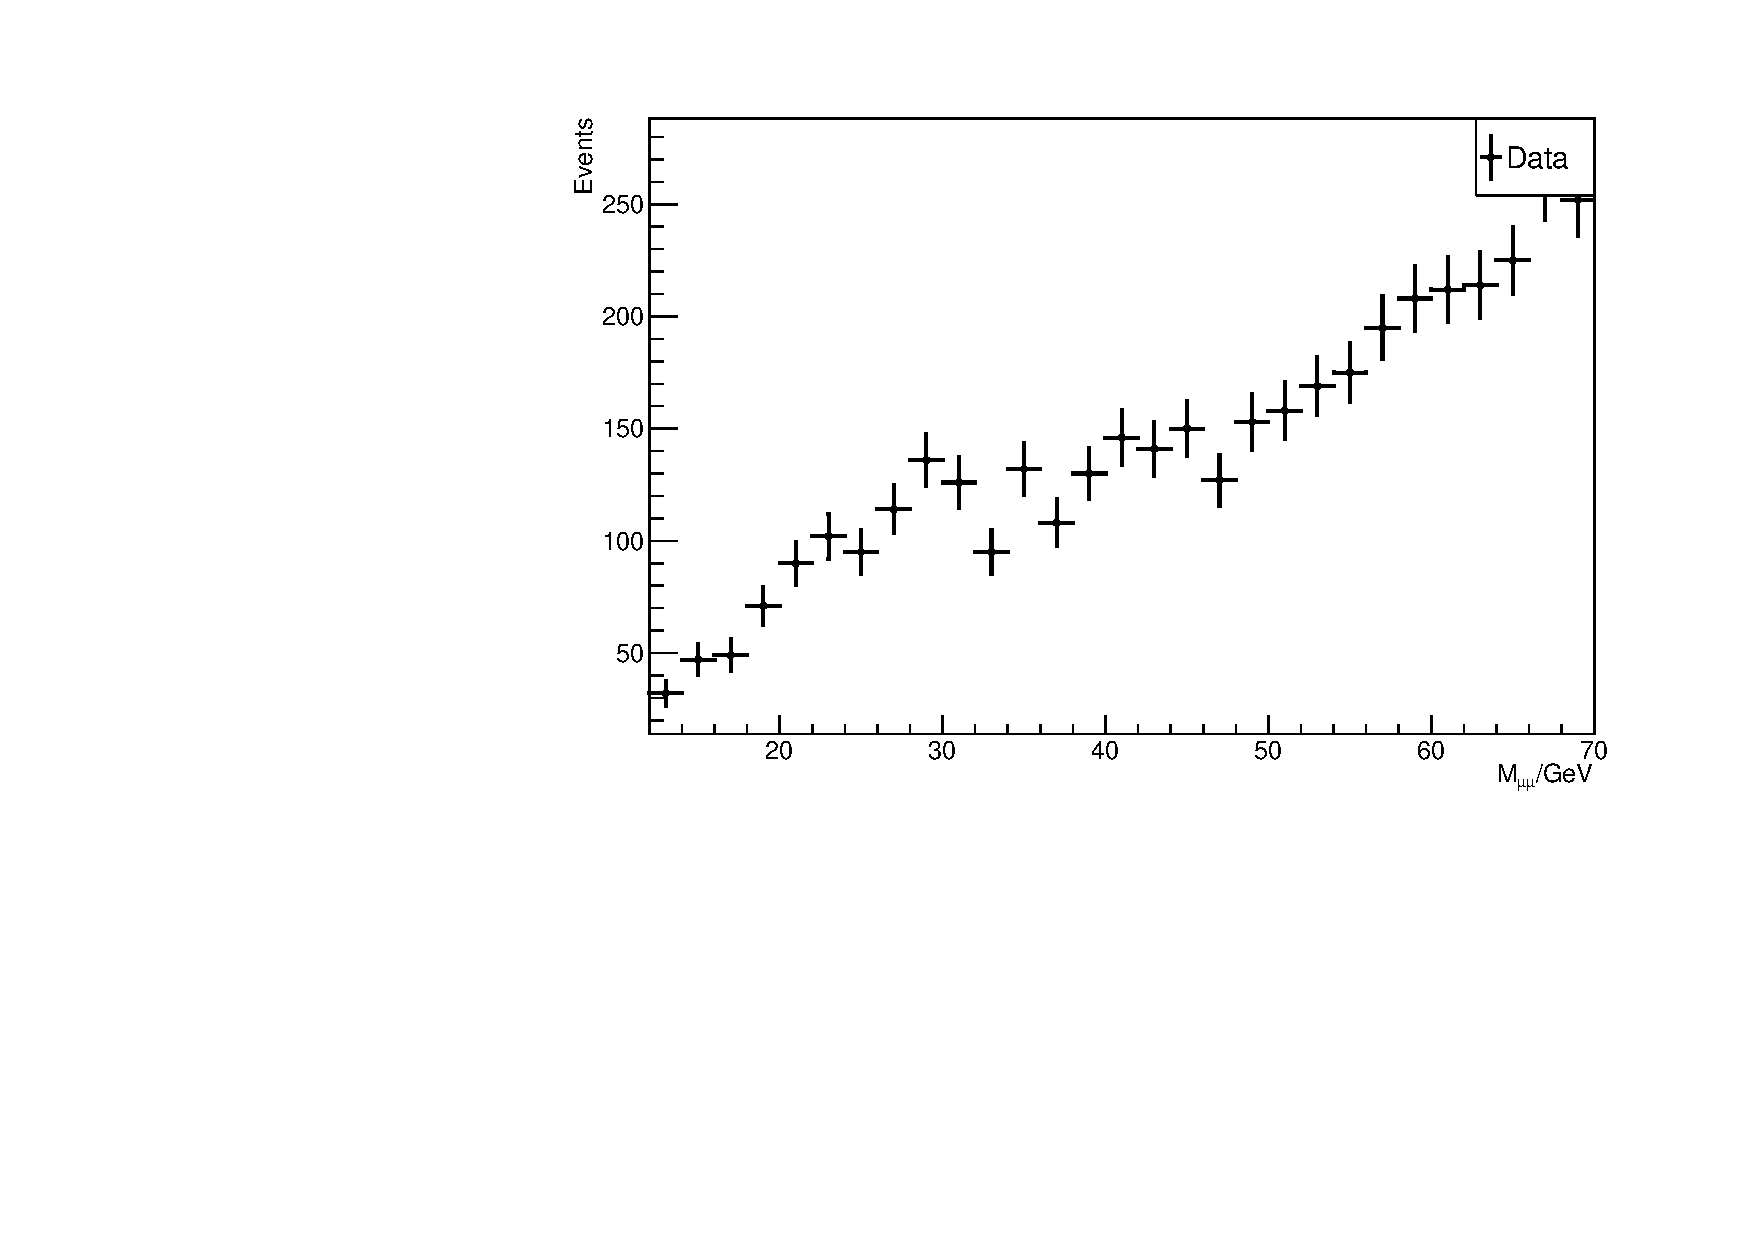
\includegraphics[width=.8\textwidth]{TalkPics/dimuoncheck100815/output_sashacheck_bugfixcsvtight/mmumu_centralbjet.pdf}
\end{frame}

\begin{frame}
  \frametitle{Dimoun mass distributions - Other central jet veto}
  \centering
  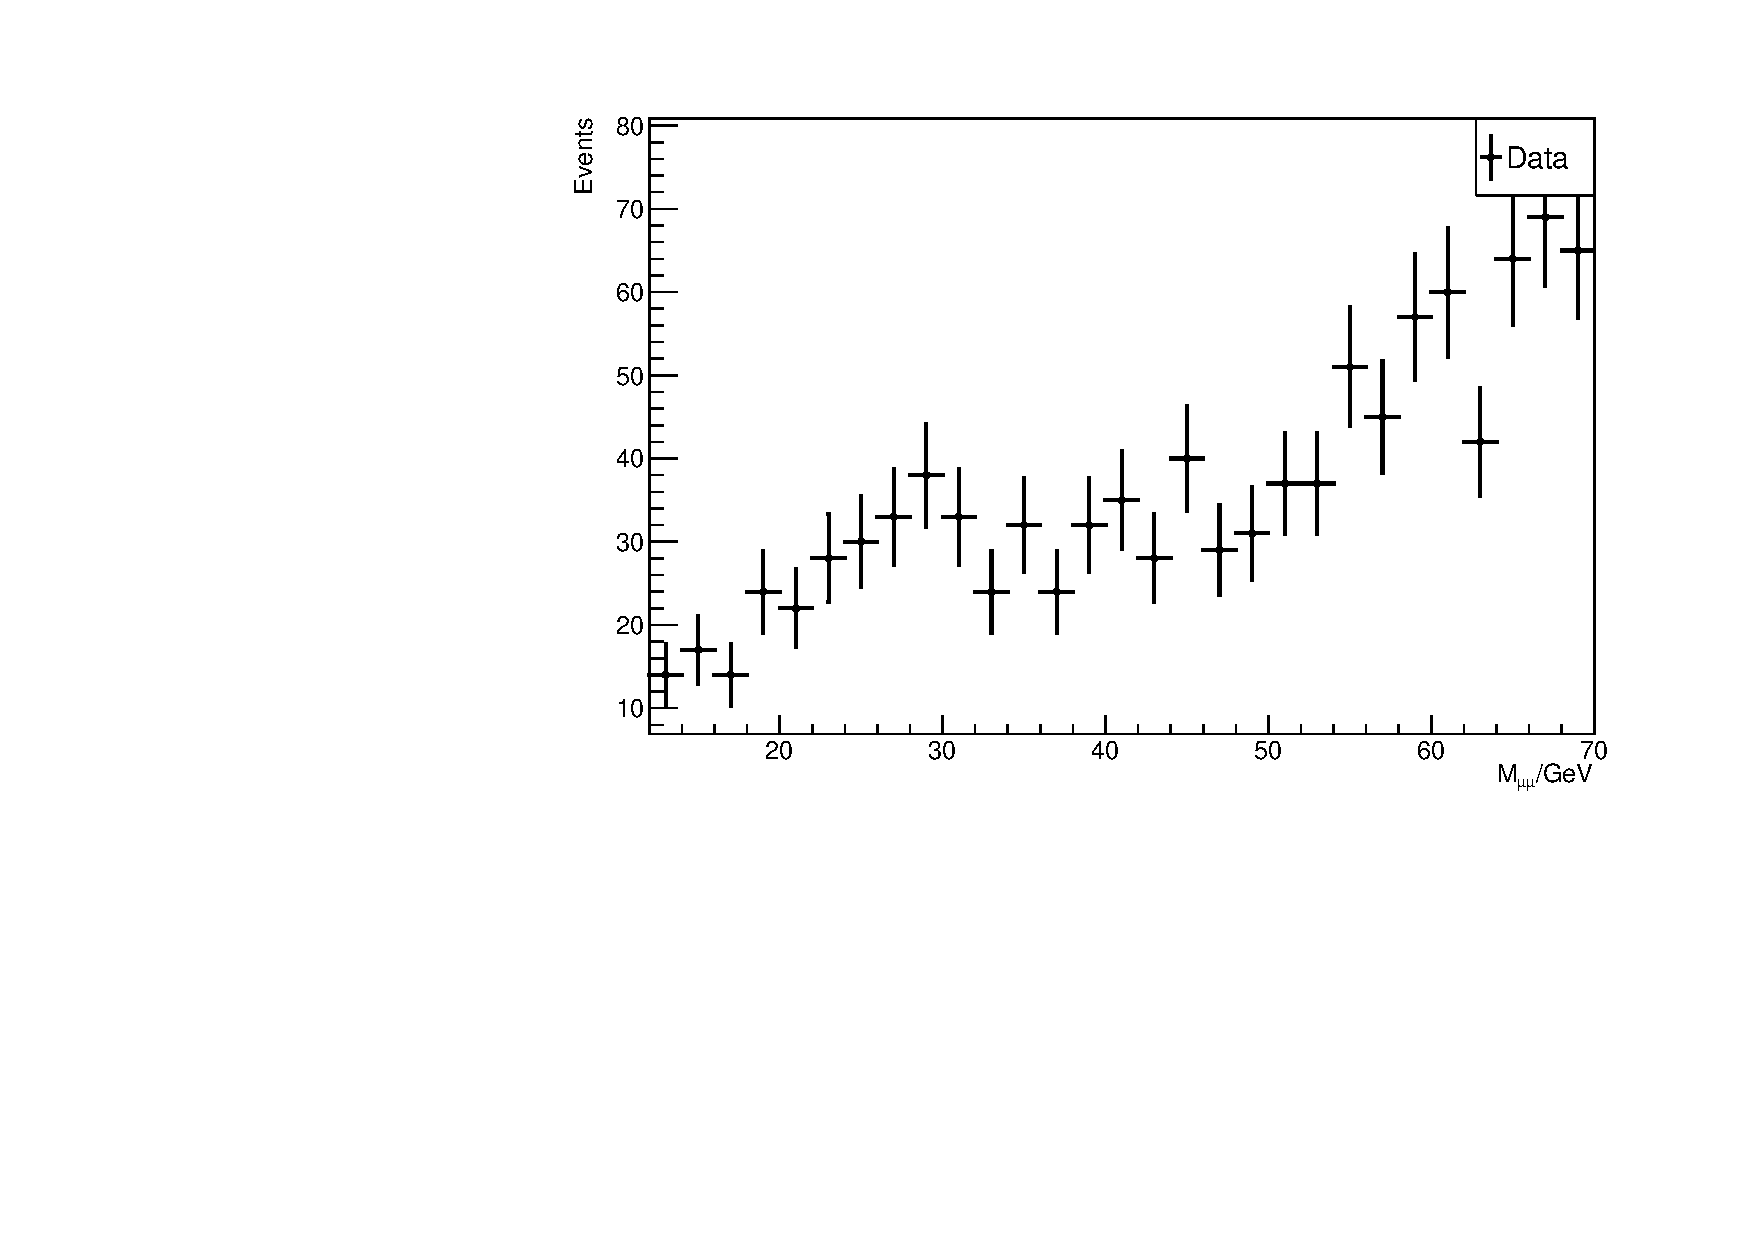
\includegraphics[width=.8\textwidth]{TalkPics/dimuoncheck100815/output_sashacheck_bugfixcsvtight/mmumu_centralbjetcjv.pdf}
\end{frame}

\begin{frame}
  \frametitle{Dimoun mass distributions - Forward jet}
  \vspace{-.3cm}
  \begin{block}{}
    \scriptsize
    \begin{itemize}
    \item Bumpy structure across whole mass range: 3 bins around 30 GeV slightly high
    \item Attempted second order polynomial plus gaussian fit:
    \item[-] No bump resolved by fit for several values of initial conditions
    \item[-] Tried 1 GeV binning, no bump at 30 GeV resolved by fit
    \end{itemize}
  \end{block}
  \centering
  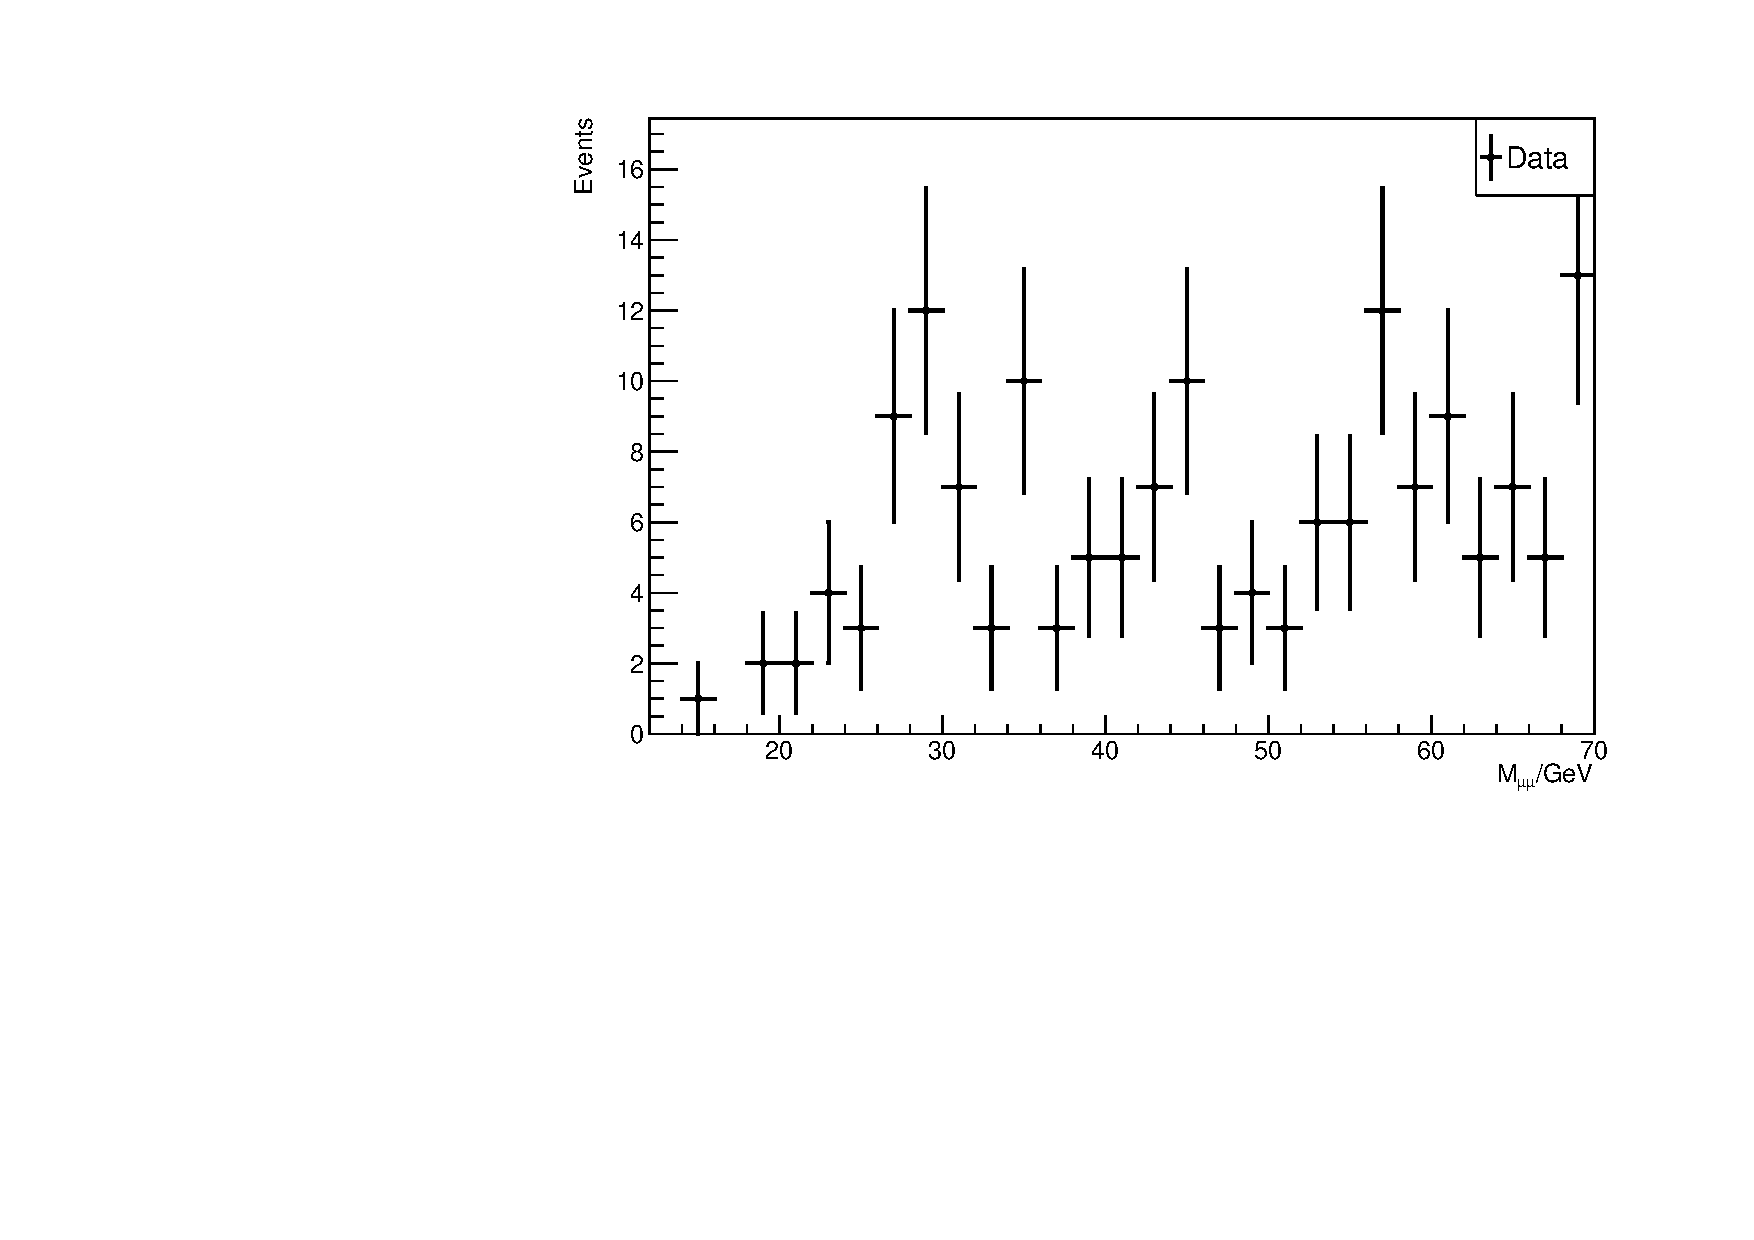
\includegraphics[clip=true,trim=0 0 0 25,width=.73\textwidth]{TalkPics/dimuoncheck100815/output_sashacheck_bugfixcsvtight/mmumu_forwardjet.pdf}
\end{frame}
%!!One slide per step
%!!forward jet cut mention pol+gaus fit doesn't 

\begin{frame}
  \frametitle{Event by event comparison}
  \begin{block}{}
    \begin{itemize}
    \item Compare events in 26-32 GeV with original analysis
    \item 10 events from original analysis fail my selection
    \end{itemize}
  \end{block}
  \begin{block}{6 events have no second muon}
      \begin{itemize}
    \item Only known muon ID difference is isolation
    \item Suggests these events pass track iso but fail pf
    \item Consistent with yields being lower from dimuon selection
    \item Efficiency difference between isolations is small $\sim \%$
    \end{itemize}
  \end{block}
\end{frame}

\begin{frame}
  \frametitle{Event by event comparison - continued}
  \begin{block}{4 events have additional central jets}
    \begin{itemize}
    \item Some overlap with above 6 events
    \item Known differences are PU ID and muon overlap veto
    \end{itemize}
  \end{block}
  \begin{block}{1 event has no b jet}
    \begin{itemize}
    \item Known different b-tag algorithm
    \end{itemize}
  \end{block}
  \begin{block}{1 event has dimuon mass outside window}
    \begin{itemize}
    \item Known MuScle fit difference
    \end{itemize}
  \end{block}
\end{frame}


\begin{frame}
  \frametitle{Summary}
  \label{lastframe}
  \begin{block}{}
    \begin{itemize}
    \item Imperial College H$\rightarrow\tau\tau/$inv. framework and ntuples have been used to crosscheck dimuon bump analysis
    \item Cut flow efficiency very similar to original analysis:
    \item[-] Yields slightly lower
    \item No bump significant enough to be resolved by a polynomial plus gaussian fit
    \item Event by event comparison suggests muon isolation and additional central jets cause differences
%!!muon isolation 
%!!Three bins around 30 GeV are slightly high but no significant excess seen

    \end{itemize}
  \end{block}
\end{frame}

\begin{frame}
  \frametitle{Backup}
\end{frame}

\end{fmffile}
\end{document}
